\section{Results}

\subsection{Data}\label{sec:results:data}

\mdeff{All stuff about data here.
Ideally same data for all experiments.}
\todo{Merge and shorten.}
\todo{$P$ training projections.}

We consider two proteins as ground truths: the $\beta$-galactosidase, a protein with a dihedral (D2) symmetry, and the lambda excision HJ intermediate (HJI), an asymmetric protein.
Their deposited PDB atomic models are 5a5a ~\cite{bartesaghi2015betagal} and 5j0n~\cite{laxmikanthan2016structure}, respectively.
For each atomic model, we generate the ground truth by fitting a 5\AA\ density map in Chimera~\cite{pettersen2004ucsf}.
We thus obtain a volume of size $(117\times 117\times 117)$ for the $\beta$-galactosidase, and a volume of size $(275\times 275\times 275)$ for the HJI.

From these ground truths, we generate $5,000$ synthetic projections of size $(117\times 117)$ and $(275\times 275)$, respectively, using the ASTRA projector~\cite{van2015astra}.
The projection orientations are sampled from a uniform distribution over half the $\SO(3)$ space, which suffices to generate all the possible projections of a volume.
For the sake of simplicity, the projections are currently kept unblurred and noiseless.
Whenever training neural networks, we split the datasets into a distinct training set (50\%), validation set (22\%), and testing set (33\%), to ensure that the results can generalize to unseen projections.
The complete pipeline is implemented in Tensorflow~\cite{abadi2016tensorflow}.

\paragraph{Generating a Proper Training Dataset for the SiameseNN}

The success of the SiameseNN as a faithful predictor of relative orientations eventually relies on our capacity to generate a synthetic training dataset that is both large and representative of SPA measurements.
In other words, we need to create a training set whose data distribution is diverse enough to cover that of unseen projection datasets.
The objective is for the SiameseNN to be able to handle projections acquired in all sorts of imaging conditions and originating from 3D volumes it has never been trained on.

We shall create such comprehensive training dataset by capitalizing on two favorable conditions.
First, there exists a large publicly-available database of deposited atomic models of proteins, which gives us access to thousands of different 3D ground truths.
Then, we shall take advantage of our ability to model the cryo-EM imaging procedure to generate, from these ground truths, a synthetic dataset that contains a massive amount of realistic projections whose orientations are, by definition, all known.

Note that an interesting aspect of SiameseNNs for the present application is that they intrinsically predict the \textit{relationship} between objects.
Hence, a well-trained SiameseNN could be relatively robust to the change of volumes.
In the same line of thought, our SiameseNN will likely benefit from the profound structural similarity shared by proteins---after all, they all derived from just the same 21 amino acids.

\subsection{Evaluation}\label{sec:results:evaluation}

\mdeff{Story: need to know how good we did (without reconstructing the protein).
As orientations are up to a global rotation/mirror on $\SO(3) / \mathbb{S}^3$, best align recovered and true orientations before computing the mean recovery error.}

\todo{Introduce the mean recovery error as a good and intuitive performance metric.}

Before discussing the results, we remark that one cannot really quantify the performance of~\eqnref{orientation-recovery} through its loss.
Unfortunately, it is also not appropriate to directly compute the error between the recovered orientations $\big\{\widehat{q}_p\big\}_{p=1}^P$ and the true ones $\big\{q_p\big\}_{p=1}^P$.
The reason is that the recovery of orientation through~\eqnref{orientation-recovery} is up to a global rotation, \textit{i.e.}, any global rotation of the set of recovered orientations is as valid as any other.
This is not a problem for the ultimate application of our scheme, but it complicates the quantitative evaluation of its performance in synthetic experiments.
We circumvent this problem by 1) aligning the true and recovered orientation sets, and 2) computing their distance after alignment.
The alignment is performed by searching for the orthogonal matrix (with determinant $\pm$ 1) $\mathbf{T}\in\mathbb{R}^4$  that minimizes
\mdeff{We don't care about $\mathbf{T}$, but about} the \textit{mean orientation recovery error}
\begin{equation}
    E = \min_{\T \in \Or(4)} \frac{1}{P^2} \sum_{i,j} \big| d_q\left(q_i,q_j\right)- d_q\left(\mathbf{T}\widehat{q}_i,\mathbf{T}\widehat{q}_j\right) \big|^2,
    \label{eqn:orientation-recovery-error}
\end{equation}
where $\Or(4) = \{\T \in \R^4 | \det(\T) = \pm 1\}$ is the group of $4 \times 4$ orthogonal matrices that represent 4D rotations and mirrors.
In practice, the sum is again sampled and \eqnref{orientation-recovery-error} is separately minimized by SGD for $\det(\T) = 1$ and $\det(\T) = -1$ because $\Or(4)$ is disconnected.
%Note the similarity with~\eqnref{metric-learning} and~\eqnref{orientation-recovery}.
\mdeff{We do normalize by the number of pairs right?}

\subsection{Orientation recovery}\label{sec:results:orientation-recovery}

\mdeff{Story: good distance estimation = good orientation recovery.}
\mdeff{(Nothing to write here.)}

%\subsubsection{Feasibility Check: Recovery from the Exact Relative Distances}
\subsubsection{Recovery from exact distances}\label{sec:results:orientation-recovery:exact}

\mdeff{Story: works perfectly despite no convexity guarantee and sampling.}
\mdeff{I made it concise but precise.
Let's do that for all!}

To verify that (i) the lack of a convexity guarantee for \eqnref{orientation-recovery} and (ii) the severe sampling of the sum are non-issues in practice, we attempt orientation recovery under exact distance estimation $d_p(\p_i, \p_j) = d_q(q_i, q_j)$.
From $P=5000$ projections taken from one side of the asymmetric protein (5j0n), we sample $5000$ out of $P^2 = \num{25e6}$ pairs and minimize \eqnref{orientation-recovery} with Adam~\cite{kingma2014adam}, a variant of SGD, for $\num{30e3}$ steps ($\sim 1$ hour) with a learning rate of $0.1$.
Orientations are perfectly recovered.
\figref{minim-loss-perfect-distances} shows the convergence of~\eqnref{orientation-recovery} to zero.

\begin{figure}
    \centering
    \begin{subfigure}[b]{0.58\textwidth}
        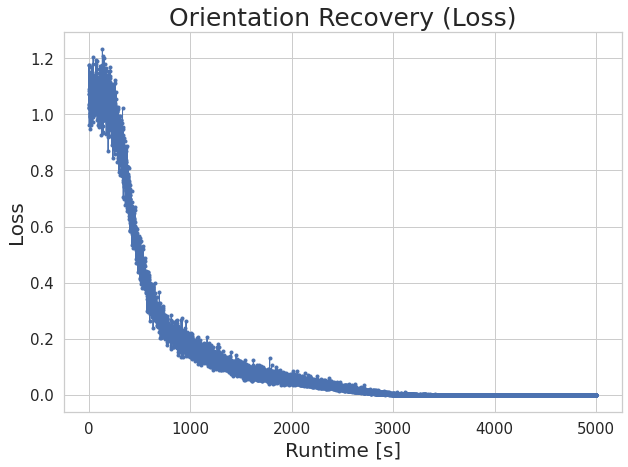
\includegraphics[height=6cm]{fig_perfectdistances_loss-symmetric}
        \caption{}
    \end{subfigure}
    \hfill
    \begin{subfigure}[b]{0.40\textwidth}
    \centering
        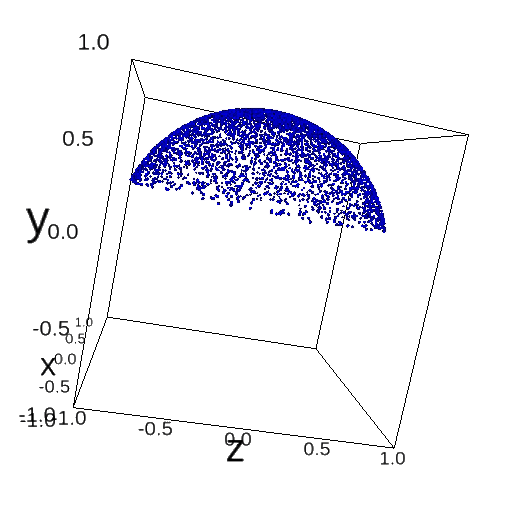
\includegraphics[height=6cm]{fig-perfectdistances-coverage-symmetric}
        \caption{}
    \end{subfigure}
    \caption{
        Orientation recovery under exact distance estimation $d_p(\p_i, \p_j) = d_q(q_i, q_j)$.
        \textbf{(a)} Evolution of objective~\eqnref{orientation-recovery}.
        \textbf{(b)} Orientation coverage of $\mathbb{S}^2 \subset \SO(3)$ after recovery.
        % orientations projected on S²
}
    \label{fig:minim-loss-perfect-distances}
\end{figure}

%\subsubsection{Robustness of Recovery to Additive Errors on the Relative Distances}
\subsubsection{Sensitivity to distance estimation error}\label{sec:results:orientation-recovery:sensitivity}

\mdeff{Story: (i) orientation recovery error is strongly linked to distance estimation error, (ii) recovery loss is a good proxy of mean recovery error.}

We now go one step further and evaluate the behaviour of~\eqnref{orientation-recovery} when the true relative distances are corrupted by  additive Gaussian noise.

The experimental conditions are the same than in the previous section, except that we add an error with increasing variance on the relative distances prior to the minimization.
The results are presented in \figref{recovery-noise-distances} (red curve).

\begin{figure}
    \centering
    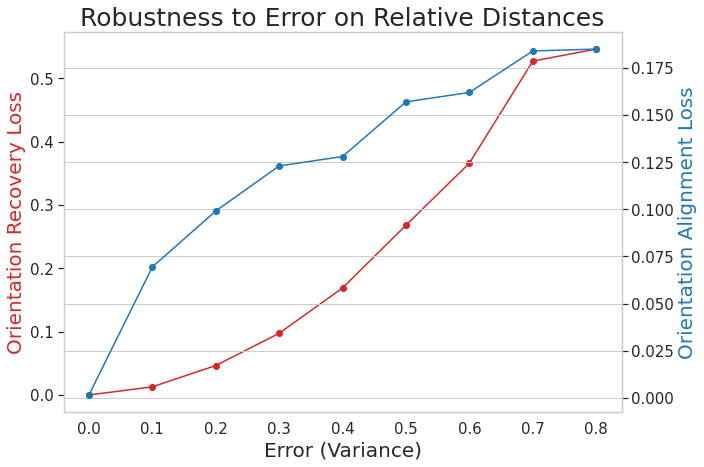
\includegraphics[width=0.75\textwidth]{fig-robustness-asymmetric}
    \caption{
        The mean orientation recovery error \todo{(eq)} is a monotonic function of the distance estimation error.
        Better distance estimation leads to better orientation recovery.
        Moreover, the recovery loss \todo{(eq)} is a good proxy for the recovery error, allowing us to assess recovery performance without ground-truth orientations.
        \todo{Figure: "variance of white noise added to true distance" as x-label.
No title.
"mean orientation recovery error [radians]" as right y-label.
Invert the two y-axes, so the red curve is close to the red label and the blue curve is close to the blue label.}
}
    \label{fig:recovery-noise-distances}
\end{figure}

For all variances, the distance after alignment is reported in \figref{recovery-noise-distances} (blue curve).

These results demonstrate that the performance of the minimization scheme~\eqnref{orientation-recovery} linearly depends on the quality of the relative distances, which advocates for a proper and extensive training of the SiameseNN in the next stages of development.
Another interesting output of \figref{recovery-noise-distances} is that it indicates that the error of the orientation recovery behaves as a monotonic function of its loss.
Hence, it suggests that the loss can be used as a good indicator of its performance, which has obvious practical implications for our future works on real data.

\subsection{Distance estimation}\label{sec:results:distance-estimation}
%\subsection{Estimating Relative Orientations from Projections}
%\subsection{Relative orientation estimation}

\mdeff{Story: $d_p$ good estimator of $d_q$.
SiameseNN better than l2, but still plateaus.
Robust to projection noise.}

\mdeff{Could we quickly try translations? Should be no problem for Siamese.}

\subsubsection{Euclidean distance}\label{sec:results:distance-estimation:euclidean}

\mdeff{Story: simplest baseline estimator, $d_{pe}$ somewhat estimates $d_q$, quickly plateaus (even in the simplest noiseless and centered case).
Note the difference between symmetric and asymmetric proteins.}

As a baseline, we first evaluate the suitability of the Euclidean distance as a projection distance $d_b$ to predict $d_q$.
For the two aforementioned datasets, we randomly select $1,000$ pairs of projections.
For each pair, we compute the Euclidean distance between the projections $d_b(\mathbf{b}^i,\mathbf{b}^j)=\lVert\mathbf{b}^i-\mathbf{b}^j\rVert_2$ and their relative orientation $d_p(q_i,q_j)$ through~\eqnref{distance:orientations}.
We then report the $(d_q,d_b)$ relationship for all pairs in \figref{euclidean-not-robust}, for both the asymmetric protein (left) and the symmetric one (right).

\begin{figure}
    \centering
    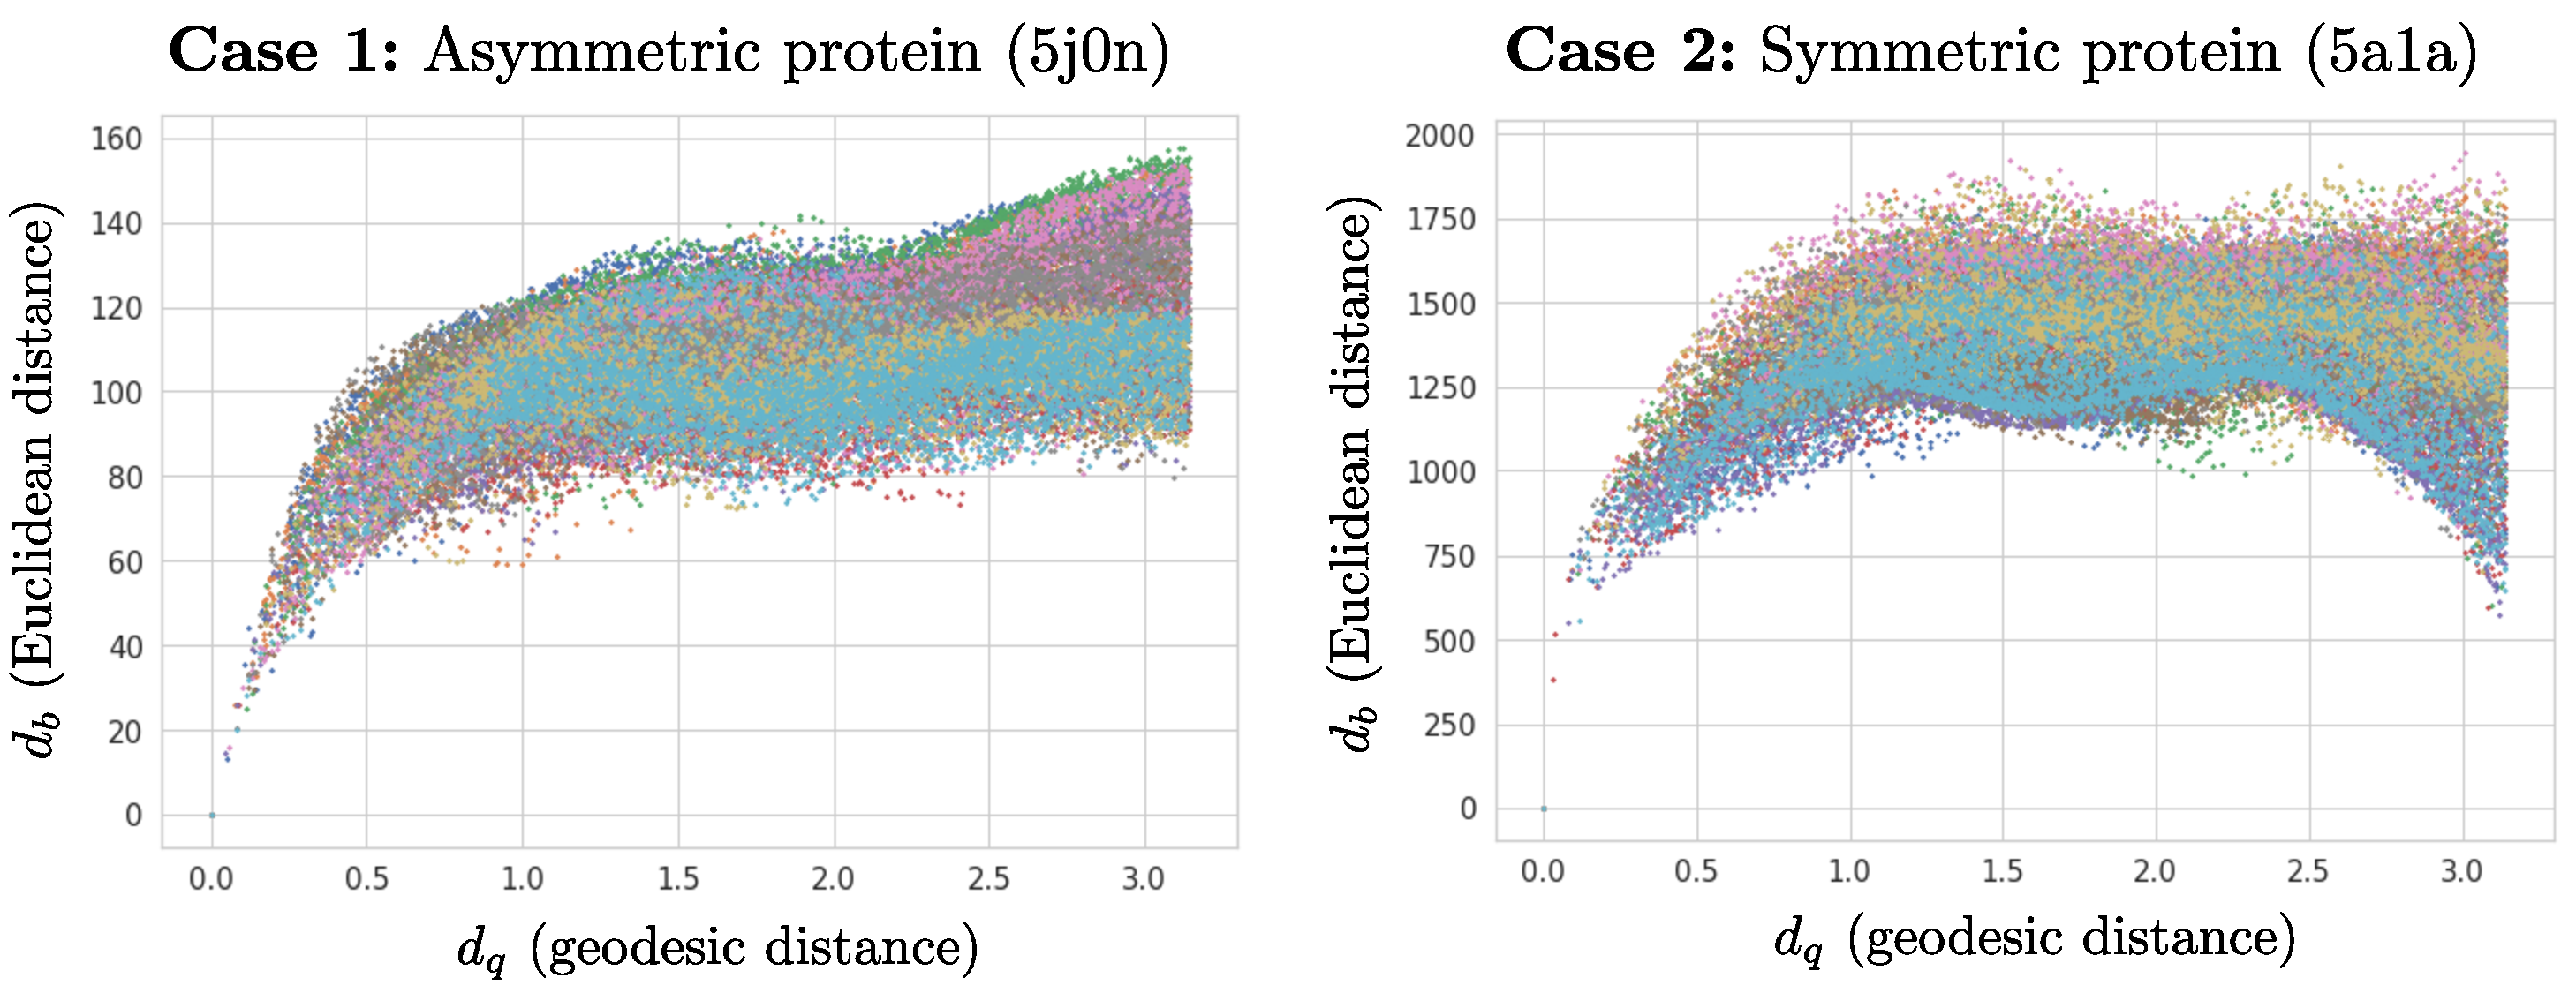
\includegraphics[width=\textwidth]{EuclideanDistance_NonRobust}
    \caption{
        Plotting the Euclidean distance between two projections versus their actual relative orientation (measured by the geodesic distance) for \textbf{(left)} the asymmetric protein (5j0n) dataset, and \textbf{(right)} the symmetric protein (5a1a) dataset.
        \todo{x-label: "geodesic distance $d_q$ between orientations".
y-label: "Euclidean distance $d_{pe}$ between projections.}
        \mdeff{What do the colors mean? Remove if irrelevant.}
    }
    \label{fig:euclidean-not-robust}
\end{figure}

Two principal observations can be made from this experiment.
First, as suspected, the Euclidean distance between projections fails to be a consistent predictor of their relative orientation distance, even in the simple imaging conditions considered here (no noise and no effect of the PSF).
In particular, the larger the relative distance $d_q$, the poorer the predictive ability of the Euclidean distance as $d_b$.
The other interesting observation is that the intrinsic symmetry of the $\beta$-galactosidase protein (5a1a) appears in its $(d_q,d_b)$ plot.

\subsubsection{Learned distance}\label{sec:results:distance-estimation:learned}

\mdeff{Story: learned distance $d_{ps}$ estimates $d_q$ with some variance but still underestimates larger distances.
Again symmetric vs asymmetric.}

\begin{figure}
    \centering
    \begin{subfigure}[t]{0.4\textwidth}
        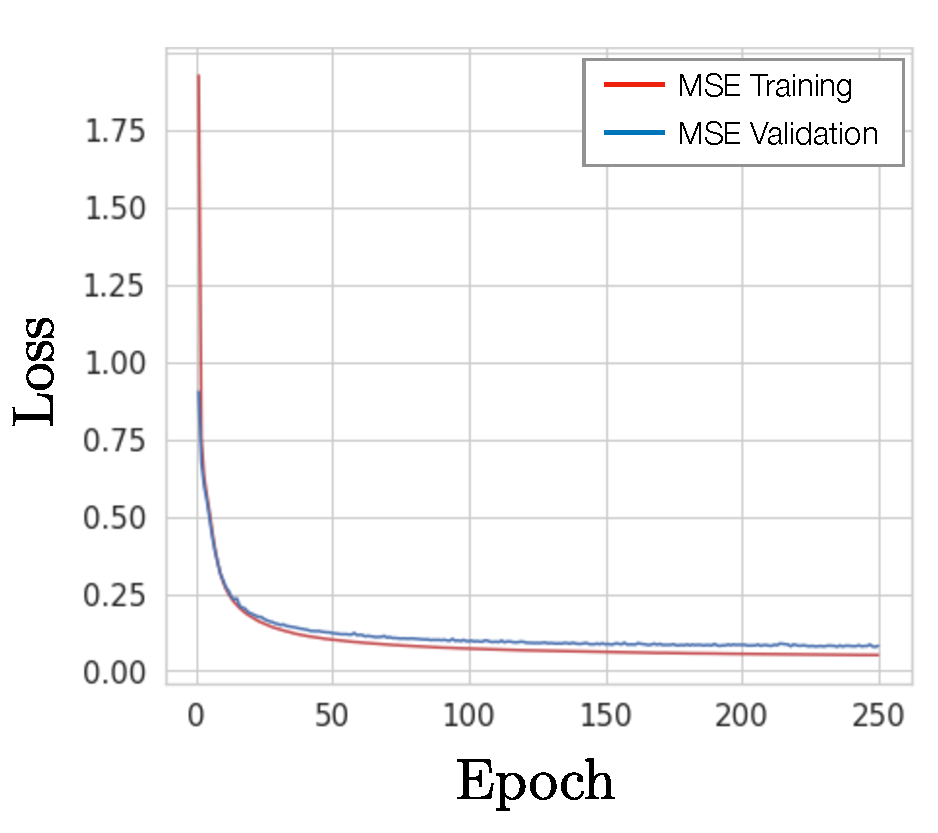
\includegraphics[width=0.98\textwidth]{TrainingSiamese_LossAssymetric}
        \caption{Training losses of the SiameseNN on the asymmetric protein (5j0n) training and validation datasets.}
        \label{fig:losses-siamese-assym}
    \end{subfigure} \quad \quad
    \begin{subfigure}[t]{0.4\textwidth}
        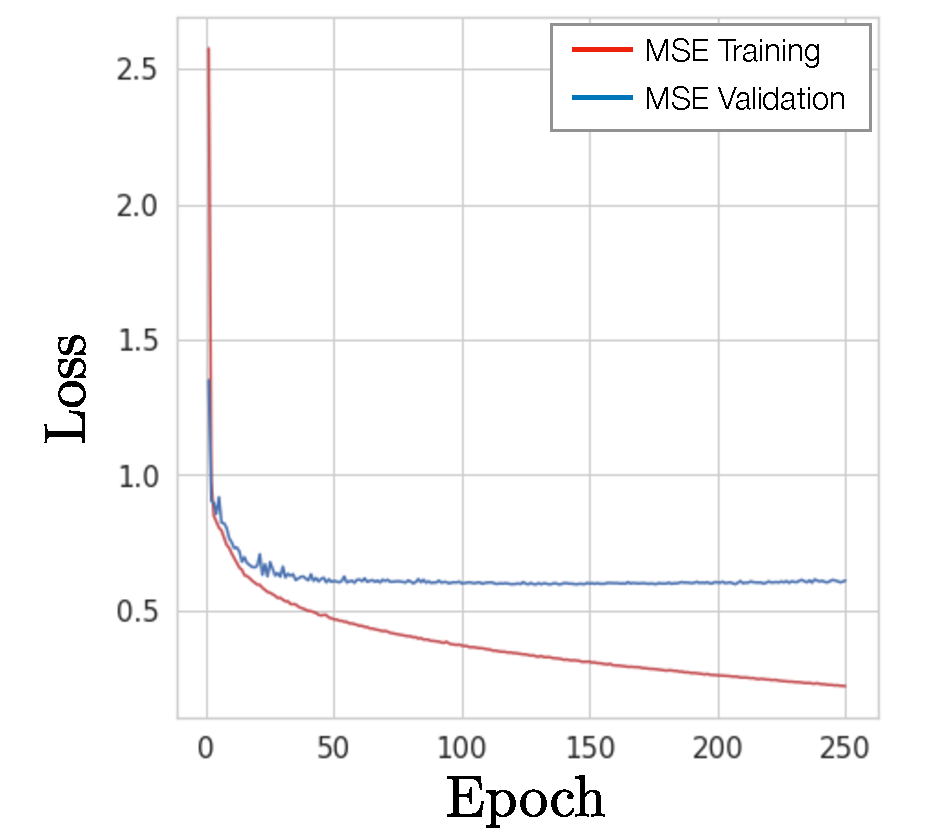
\includegraphics[width=0.98\textwidth]{TrainingSiamese_LossSymetric}
        \caption{Training losses of the SiameseNN on the symmetric protein (5a1a) training and validation datasets.}
        \label{fig:losses-siamese-sym}
    \end{subfigure} \vspace{0.45cm}
    \begin{subfigure}[t]{0.4\textwidth}
        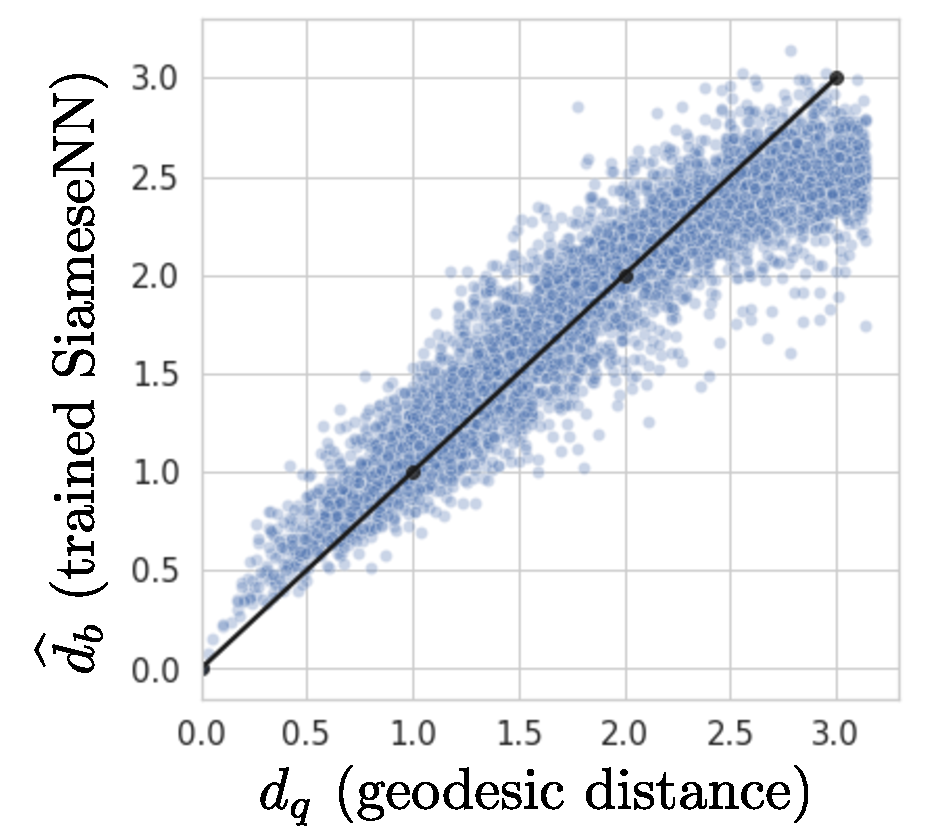
\includegraphics[width=0.98\textwidth]{TrainingSiamese_PlotAssymetric}
        \caption{Relative orientations predicted by the trained SiameseNN from projections in the asymmetric protein (5j0n) testing dataset.
}
        \label{fig:learned-distance-siamese}
    \end{subfigure} \vspace{0.35cm}
    \caption{Training results for the SiameseNN.}
    \label{fig:losses-siamese}
\end{figure}

We present here a preliminary evaluation of the ability of SiameseNNs to learn a projection distance $\widehat{d}_b$ that correctly approximates the orientation distance $d_q$.

SiameseNNs come with a variety of more or less powerful architectures.
At the current stage of development, we work with a simple one.
Our SiameseNN is composed of two convolutional neural networks (CNNs) with shared weights.
Their output features vectors are compared through an Eulidean distance, \textit{i.e.}, $F(\mathbf{x},\mathbf{y})=\lVert \mathbf{x}-\mathbf{y}\rVert_2$ in \figref{schematic:distance-learning}.
\todo{The detailed architecture of the SiameseNN is given in figref.}
\todo{$d_f$ could be parametrized as an MLP, a general function approximator.}

For each protein, we train the SiameseNN on its training dataset for 250 epochs ($\sim$10 hours) using an Adam optimizer~\cite{kingma2014adam}, a learning rate of $10^{-3}$, and a batch size of 256 projections.
The evolution of the training and validation losses are presented in \figref{losses-siamese-assym} for the asymmetric protein (5j0n), and in \figref{losses-siamese-sym} for the symmetric one (5a1a).
The results demonstrate that the SiameseNN succeeds at learning a proxy distance for the asymmetric protein dataset, as convergence is reached in about 50 epochs ($\sim$ 2 hours).

However, the current SiameseNN architecture fails at learning the distance for the dataset 5a1a, which is very likely due to the symmetry of the $\beta$-galactosidase protein.
Indeed, its synthetic dataset contains pairs of projections that share the same $d_b$, yet differ in their $d_q$.
This simply advocates for the restriction to non-overlapping areas on $\SO(3)$ when sampling the orientations used to generate the SiameseNN training dataset.
The latter would then only contain projection pairs with a linear $(d_q,d_b)$ relationship, which should ensure a successful training of the network.
For the rest of the experiments, we use the asymmetric protein (5j0n) dataset.

We then feed to the trained SiameseNN $1,000$ pairs of projections randomly selected from the 5j0n testing dataset, and report the $(d_q,\widehat{d}_b)$ relationship of each pair in \figref{learned-distance-siamese}.
These results confirm that, for this protein at least, the SiameseNN is able to predict the orientation distance $d_q$ using only the projections as inputs.
Moreover, it clearly outperforms the Euclidean distance at doing so.
These preliminary results are encouraging, as much has yet to be gained from improving upon the rather primitive SiameseNN architecture we currently use.

\subsubsection{Influence of network architecture and feature distance}

\mdeff{Story: $d_f = d_q$ better than Euclidean and MLP $d_f$. Architecture of $G_w$ doesn't seem to matter much. Surprising, because we don't overfit $\rightarrow$ future research needed.}

\subsubsection{Sensitivity to perturbed projections}\label{sec:results:distance-estimation:sensitivity}

\mdeff{Story: learned distance is minimally sensible to perturbations (additive noise, translation, PSF) because we can train it to ignore irrelevant information.
Thanks again to good model of cryo-EM imaging.}
\mdeff{Better word? (perturbations, quality, non-ideal)}

\subsection{Orientation recovery from estimated distances}

\mdeff{Story: pipeline works but better distance estimation is needed for SOTA reconstruction.
Method is however promising because learned distance is robust to perturbations and recovery works if distance works.}

\todo{Justify threshold because of plateau (figref).
Show recovered orientations w.r.t.\ ground truth after alignment.}

\todo{Reconstruct the protein to show the full pipeline: from a set of projections to a reconstructed protein.
Emphasize that it's a naive reconstruction algorithm.}
